\documentclass{scrartcl}

\usepackage{url}
\usepackage{graphicx}
\usepackage{amsmath}
\usepackage{varwidth}
\usepackage[dvipsnames]{xcolor}
\usepackage{algorithm}
\usepackage{algpseudocode}
\usepackage{listings}
\lstset{
	basicstyle=\footnotesize\ttfamily,
	tabsize=4,
	showstringspaces=false,
	breaklines=true,
	prebreak={\space\hbox{\textcolor{Gray}{$\hookleftarrow$}}},
	language=C++
}
\usepackage{enumitem}

\usepackage{tikz}
\usetikzlibrary{shapes.geometric, arrows}

\tikzstyle{flowchartnode} = [rectangle, minimum height=0.8cm, text centered, text width=3cm, draw=black, font=\small]
\tikzstyle{startstop} = [flowchartnode, rounded corners=0.4cm]
\tikzstyle{process} = [flowchartnode]
\tikzstyle{io} = [flowchartnode, trapezium, trapezium left angle=70, trapezium right angle=110, text width=2cm]
\tikzstyle{decision} = [flowchartnode, diamond, aspect=2, text width=2cm]
\tikzstyle{arrow} = [thick,->,>=stealth]

\makeatletter
\@addtoreset{section}{part}
\makeatother  

\title{Worksheet 5}
\subtitle{COMP110: Principles of Computing}
\author{Ed Powley}
\date{February 2016}

\renewcommand\thepart{\Alph{part}}

\begin{document}

\maketitle

\section*{Introduction}

\begin{figure}%
\begin{center}%
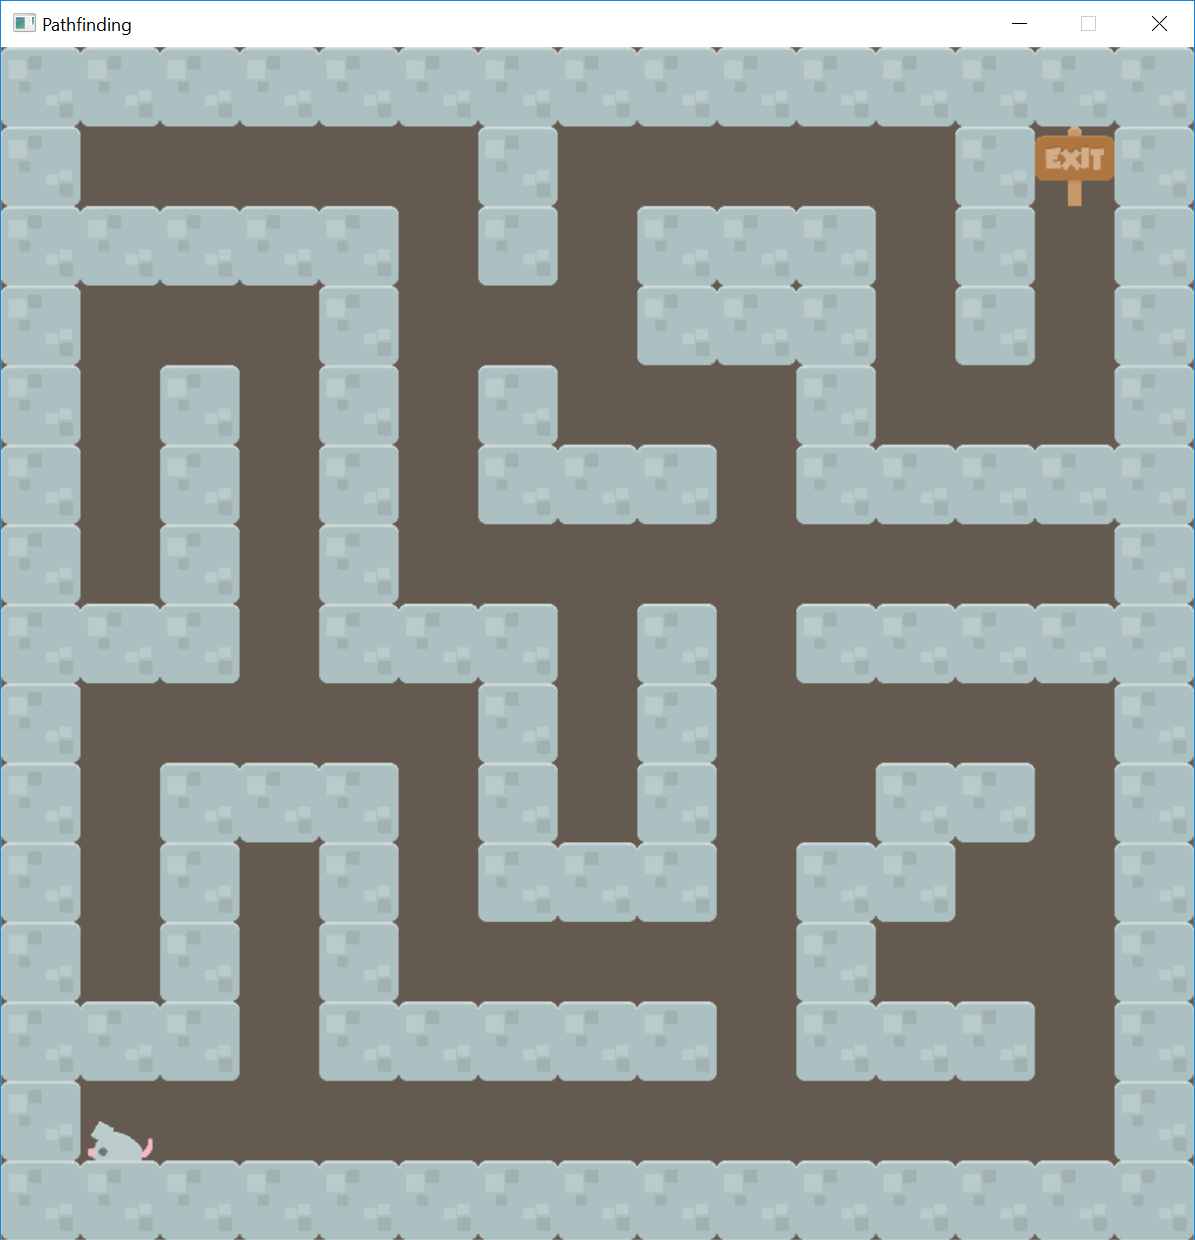
\includegraphics[width=0.4\columnwidth]{application}%
\end{center}%
\caption{A screenshot of the skeleton project.}%
\label{fig:application}%
\end{figure}

In this assignment, you will implement the \textbf{A$^*$ pathfinding algorithm} within a provided template application.

This worksheet tests your ability to translate a complex algorithm, given as pseudocode, into C++ code,
with appropriate choices of data structures.

\section*{Submission instructions}

The GitHub repository at the following URL contains the skeleton project for this worksheet.
\begin{center}
\url{https://github.com/Falmouth-Games-Academy/comp110-worksheet-5}
\end{center}
Fork this repository into your own GitHub account. To submit, create a GitHub pull request.

\textbf{Please do not rename or delete the project or files provided, and please do not create new projects.}
This will ensure that GitHub's ``diff'' view highlights only the parts of the code that you have edited.
Creating new source and/or header files is permitted, if doing so improves the structure of your programs.

\section*{Marking}

\subsection*{Timely submission: $40\%$}

The deadline for this worksheet is \textbf{6pm, Wednesday 9th March 2016}.
To obtain the marks for timely submission, you must submit (as a GitHub pull request) your progress towards the worksheet by this time.
As with other worksheets, you may resubmit after these deadlines in order to collect extra correctness or quality marks.
This $40\%$ is awarded as long as you submit \emph{something} by the deadline,
even if your submission has bugs or other issues.

\subsection*{Correctness: $30\%$}

To obtain the marks for correctness, you must submit a working solution.
Note that this is a threshold: the full $30\%$ is awarded for work which is \emph{complete}
and contains \emph{no clear errors}. In particular you will not be penalised for trivial errors which do not
affect the overall functioning of your program, nor will you receive extra credit for a highly polished solution.

\subsection*{Quality: $30\%$}

The extra quality criteria for this worksheet are as follows. All are weighted equally, so each is worth $6\%$ of the overall mark for this worksheet, with the exception of the \textbf{stretch goal} which is worth $12\%$.
\begin{enumerate}
\item\textbf{Presentation.} Your solutions are appropriately presented in GitHub, with descriptive commit messages
	and appropriate documentation in \texttt{readme.md} files.
	You have edited the provided skeleton projects, and refrained from renaming the provided files or creating new projects.
    You have checked code into GitHub regularly whilst working on the worksheet.
\item\textbf{Code quality.} Your code is well formatted.
    Variable and function names are clear and descriptive.
    Comments are used where appropriate, and are well written.
    Your formatting, naming and commenting follow consistent conventions.
\item\textbf{Choice of data structures.} You have chosen appropriate data structures for your implementation,
    and have justified your choices in the \texttt{readme.md} file.
\item\textbf{Stretch goal (weighted double).} You have submitted a working solution for the Stretch Goal task.
\end{enumerate}

\clearpage

\section*{The task}

The skeleton project provides code to load a simple maze from a text file, and display it on screen using SDL
(Figure~\ref{fig:application}).
\textbf{Implement} the function \lstinline!Pathfinder::findPath! in \texttt{Pathfinder.cpp}
to find the shortest path from the start (the mouse) to the goal (the exit sign).
Base your implementation on the pseudocode for the A$^*$ algorithm provided in Algorithm~\ref{alg:astar}.
The skeleton project is already set up to call \lstinline!Pathfinder::findPath! and display the result on screen.

A selection of test maps is provided in the \texttt{Maps} directory,
and can be chosen between by changing the constant definition near the top of \texttt{PathfindingApp.cpp}.
Make sure that your implementation works for all the provided maps.

You should pay particular attention to your choice of \textbf{data structures}.
The C++ Standard Template Library (STL) provides many standard data structures such as
vectors, linked lists, sets, maps, queues, priority queues and stacks.
Research these, consider which operations are most frequent on the collections of nodes used by the algorithm,
and choose appropriately.
\textbf{Briefly} justify your choices of data structures in your \texttt{readme.md} file.

You are strongly encouraged to make use of \textbf{object oriented programming} concepts for this task.
At the very least, you will probably want to define your own \lstinline!Node! class.
Add your own fields and methods to the \lstinline!Pathfinder! class
to improve the readability of your \lstinline!findPath! implementation.

\begin{algorithm}
	\begin{algorithmic}[1]
        \newcommand{\startNode}{\operatorname{startNode}}
        \newcommand{\goalNode}{\operatorname{goalNode}}
        \newcommand{\currentNode}{\operatorname{currentNode}}
        \newcommand{\neighbourNode}{\operatorname{neighbourNode}}
        \newcommand{\cameFrom}{\operatorname{cameFrom}}
        \newcommand{\closedSet}{\operatorname{closedSet}}
        \newcommand{\openSet}{\operatorname{openSet}}
        \newcommand{\dist}{\Call{EuclideanDistance}}
        \newcommand{\thePath}{\operatorname{path}}
        
		\Procedure{A$^*$}{$\startNode, \goalNode$}
			\State $\closedSet \gets \{\}$
            \State $\openSet \gets \{\startNode\}$
            \State $\startNode.g \gets 0$
            \State $\startNode.h \gets \dist{\startNode, \goalNode}$
            \State $\startNode.\cameFrom \gets \operatorname{null}$
            \Statex
			\While{$\openSet$ is not empty}
                \State $\currentNode \gets$ node in openSet with lowest $g + h$ score
                \If{$\currentNode = \goalNode$}
                    \State \textbf{return} \Call{ReconstructPath}{$goalNode$}
                \EndIf
                \Statex
                \State remove $\currentNode$ from $\openSet$
                \State add $\currentNode$ to $\closedSet$
                \Statex
                \For{each $\neighbourNode$ adjacent to $\currentNode$}
                    \If{$\neighbourNode$ is not a wall \textbf{and} $\neighbourNode$ not in $\closedSet$}
                        \State $g_{\text{tentative}} \gets \currentNode.g
                            + \dist{\currentNode, \neighbourNode}$
                        \If{$\neighbourNode$ not in $\openSet$
                                \textbf{or} $g_{\text{tentative}} < \neighbourNode.g$}
                            \State $\neighbourNode.g = g_{\text{tentative}}$
                            \State $\neighbourNode.h \gets \dist{\neighbourNode, \goalNode}$
                            \State $\neighbourNode.\cameFrom \gets \currentNode$
                            \State add $\neighbourNode$ to $\openSet$ (if it is not already in)
                        \EndIf
                    \EndIf
                \EndFor
			\EndWhile
            \Statex
			\State \textbf{return} ``Failed to find a path''
		\EndProcedure
        \Statex
        \Procedure{ReconstructPath}{$\goalNode$}
            \State $\thePath \gets \{\}$
            \State $\currentNode \gets \goalNode$
            \While{$\currentNode \neq \operatorname{null}$}
                \State add $\currentNode$ to the beginning of $\thePath$
                \State $\currentNode \gets \currentNode.\cameFrom$
            \EndWhile
            \State \textbf{return} $\thePath$
        \EndProcedure
	\end{algorithmic}
    \caption{The A$^*$ algorithm}
    \label{alg:astar}
\end{algorithm}

\section*{Stretch goal}

\textbf{Adapt} your program to visualise the operation of the A$^*$ algorithm.
At each step of the algorithm, your program should display at least:
\begin{itemize}
    \item The \textbf{current node};
    \item The \textbf{partial path} from the start node to the current node;
    \item Which nodes are in the \textbf{open set};
    \item Which nodes are in the \textbf{closed set}.
\end{itemize}

If you attempt this part, do so in a new \textbf{branch} within your GitHub repository:
your basic A$^*$ implementation should remain in the \texttt{master} branch,
and your visualisation should be in the new branch.

\end{document}
